\chapter{評価}
\label{evaluation}

本章では、~\ref{implementation}章で述べたTreeSwiftを用いて、現行のSwiftコンパイラとその構文解析器の複雑性に関する比較評価を行う。

\section{評価手法}
\label{evaluation:method}

~\ref{implementation:part}節で述べたように、本評価では各コンパイラの複雑性を比較した上で比較結果の原因となった箇所を特定することを目的とする。
そのために、コンパイラの構文解析器のみに着目し、特定のプログラムをコンパイルするために必要な箇所のみ抜き出してその複雑性を評価する。

表~\ref{table:evaluation-property}に、~\ref{readability:evaluation}節の各手法について、構文解析器のみを対象とし(条件A)、さらにその中の特定の実行パスだけを抜き出したものを対象とする(条件B)という2つの条件下でも考察するに値する結果が得られる見込があるかをまとめた。
LOCはその計測の容易さから部分的なプログラムでも正確に計測を行い、考察に繋げることができると考えられるが、他の手法はソフトウェア全体の複雑性を包括的に捉えることを目的としているため、本評価で用いるには適切とはいえない。

そのため、本研究ではLOCに基づいて、表~\ref{table:complexity-measure}に示す手順で計測を行う。
この手順によって、図~\ref{img:loc-measurement}のように特定のプログラムを実行した場合のコードだけを対象として計測を行うことができる。
この手順で計測された値は通常のLOCとは異なるため、これ以降区別するために実行部分LOCと呼ぶ。

\begin{table}[!hbtp]
    \begin{center}
        \caption{各複雑性計測手法の評価目的との合致性}
        \begin{tabular}{|p{0.1\linewidth}|p{0.1\linewidth}|p{0.1\linewidth}|p{0.65\linewidth}|}
            \hline
            評価手法 & (条件A) & (条件B) & 理由\\
            \hline
            \hline
            LOC & ○ & ○ & 行数は対象に関わらず計測が可能であり、同じように加工された2つのプログラムに対してであればそれらを比較することもできる。\\
            \hline
            FP & × & × & 比較する2つのコンパイラはデータの入出力に関して全く同じ動作をするため、比較にならない。\\
            \hline
            HCM & ○ & △ & プログラムの一部分だけを対象とした場合にHCMの値がどのような意味を示すかを慎重に考える必要がある。\\
            \hline
            CCM & ○ & × & プログラムの一部分だけを取り出すと、分岐の片方だけが実行されたプログラムでは分岐があるにも関わらず異なる実行パスが存在しないので、CCMの値の意味が変化してしまう。\\
            \hline
        \end{tabular}
        \label{table:evaluation-property}
    \end{center}
\end{table}

\begin{table}[!hbtp]
    \begin{center}
        \caption{実行時LOCの計測手順}
        \begin{tabular}{|p{0.05\linewidth}|p{0.9\linewidth}|}
            \hline
            順番 & 手順 \\
            \hline
            \hline
            1 & 計測対象のコンパイラを構文解析のみを実行するように変更し、デバッグ情報付きでコンパイルする \\
            \hline
            2 & コンパイラをデバッガで読み込み、ソースコード中のすべての行にブレークポイントを追加する \\
            \hline
            3 & ブレークポイントは対応する機械語の存在する行でのみ設定されるため、その数を数える \\
            \hline
            4 & 1で用意したコンパイラを評価用のSwiftプログラムに対して実行し、1度でもヒットしたブレークポイントに印をつける \\
            \hline
            5 & 印のついたブレークポイントの数を数える \\
            \hline
        \end{tabular}
        \label{table:complexity-measure}
    \end{center}
\end{table}

\begin{figure}
    \begin{center}
        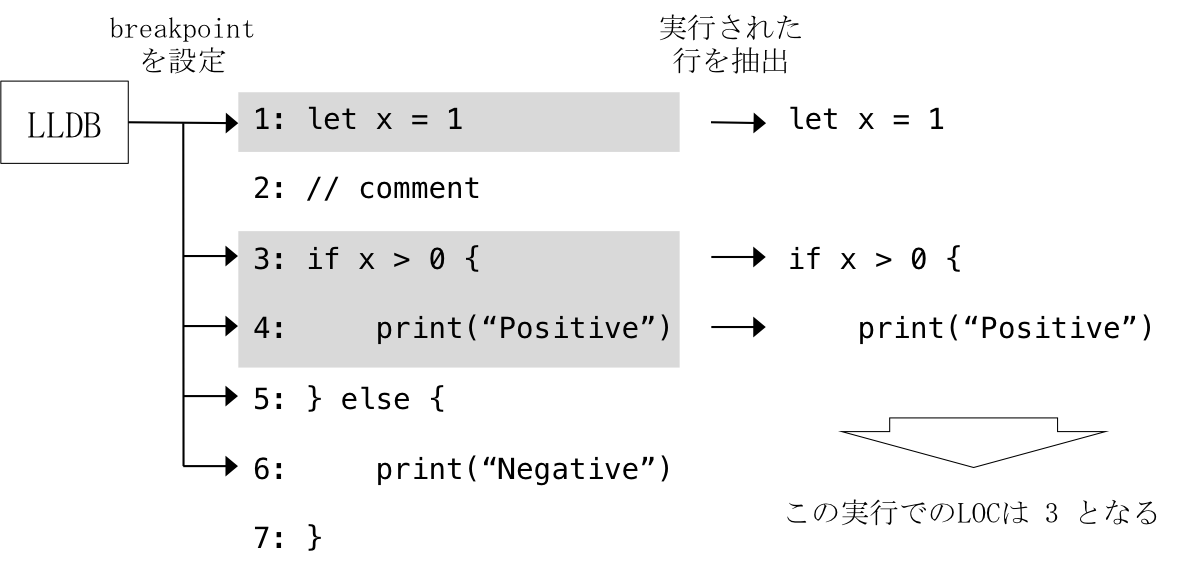
\includegraphics[scale=0.8]{./img/loc_measurement.png}
        \caption{実行部分LOCの計測手順}
        \label{img:loc-measurement}
    \end{center}
\end{figure}

現行のSwiftコンパイラについては、もともと用意されている構文解析のみを実行するオプションをつけるだけでなく、通常そのオプションと共に有効化されるASTの表示機能をコメントアウトすることで、構文解析のみが確実に実行されるように調整している。
また、コンパイラを読み込むデバッガは両コンパイラ共にLLDBのバージョン340.4.119を使用している。
具体的に評価で使用しているSwiftコンパイラおよびその実行時オプションの詳細は表~\ref{table:swift-executable}にまとめている。
なお、~\ref{implementation:abstract:parser}節で述べたようにTreeSwiftと現行のSwiftコンパイラではモジュールファイルの形式が異なっており、その点が結果に影響する可能性があるため、計測時にはコンパイラへ標準ライブラリのパスを与えず、モジュールファイルの解析に関する部分が計測対象に含まれないようにしている。

\begin{table}[!hbtp]
    \begin{center}
        \caption{評価に使用したSwiftコンパイラの詳細情報}
        \begin{tabular}{|p{0.3\linewidth}|p{0.65\linewidth}|}
            \hline
            バージョン & swift-2.2-SNAPSHOT-2015-12-31-a からASTの表示をコメントアウトしたもの\\
            \hline
            実行時に使用するオプション & -frontend -dump-parse\\
            \hline
        \end{tabular}
        \label{table:complexity-measure}
    \end{center}
\end{table}

計測時にコンパイラに読ませるSwiftプログラムにはApple社が提供するプログラミング言語Swiftのチュートリアル~\cite{swift-tour}で用いられている7つのサンプルプログラムを使用する。
ただし、これらのサンプルプログラム中に含まれていた文字リテラル中への式の埋め込みとクロージャを引数に取る関数呼び出しでの括弧の省略のみについてはTreeSwiftが対応していないため、同じ意味を持つ明示的な文字列への変換および文字の結合と括弧付きの呼び出しに変更している。
各プログラムの概要を表~\ref{table:measure-sample-programs}にまとめた。
これらのプログラムはチュートリアルという特性上Swiftの代表的な機能を充分網羅している上、プログラムで使用される変数や型に使用する名前や値、処理の構造には実際のソフトウェアを想定したような現実的なものが選ばれているため、コンパイラの機能を満遍なく使いつつも特に実際のソフトウェアでもよく用いられるであろう箇所にフォーカスした計測ができると期待できる。

\begin{table}[!hbtp]
    \begin{center}
        \caption{計測に使用するSwiftプログラム}
        \begin{tabular}{|p{0.4\linewidth}|p{0.1\linewidth}|p{0.45\linewidth}|}
            \hline
            ファイル名 & コメントや空行を除いた行数 & プログラムの概要\\
            \hline
            \hline
            simple\_values.swift & 25 & 変数の定義と使用、文字・数値・配列・辞書リテラルの使用について説明されている。\\
            \hline
            control\_flow.swift & 67 & 分岐や繰り返しについて、Swiftに特徴的なオプショナル値やパターンマッチと組み合わせた例を中心に説明されている。\\
            \hline
            functions\_and\_closures.swift & 69 & 関数の定義と使用について、基本的なものから可変長引数やクロージャを用いた高階関数の呼び出しなどの応用的なものまでが説明されている。\\
            \hline
            objects\_and\_classes.swift & 82 & クラスとそのインスタンス化、継承、関数のオーバーライドなどのSwiftにおけるオブジェクト指向プログラミングについて説明されている。\\
            \hline
            enumerations\_and\_structures.swift & 62 & 構造体とSwiftに特徴的な関数や関連型などを持つ事のできる列挙体についてその宣言方法と使い方が説明されている。\\
            \hline
            protocols\_and\_extensions.swift & 33 & 存在型や型拡張によるクラスや構造体の分類および拡張について説明されている。\\
            \hline
            generics.swift & 25 & 型パラメータ多相を用いた関数や列挙体の宣言方法とその使用方法について説明されている。\\
            \hline
        \end{tabular}
        \label{table:complexity-measure}
    \end{center}
\end{table}

\section{計測}
\label{evaluation:measure}

まず、表~\ref{table:complexity-measure}の各プログラムをコンパイルした場合それぞれについて~\ref{evaluation:method}節で説明した方法を用いて実行部分LOCを計測した。
表~\ref{table:loc-result}がその結果および現行のSwiftコンパイラの結果(表中Swift)をTreeSwiftの結果(表中TreeSwift)で割った値の一覧である。
単純に計測結果だけを見ると、プログラムのコンパイルに要した行数は現行のSwiftコンパイラの方が2\~3倍近く多い。
ただし、TreeSwiftではSwiftコンパイラとして必要な構文解析以外の処理が全て実装されているわけではないため、SwiftコンパイラにおいてはASTの検査など後の処理のための準備が行われており、実行部分LOCが大きく算出されている可能性がある。

そのため、次に各コンパイラの結果をソースコードのファイルごとに分けた上で、構文解析の本体を構成するファイル(構文解析本体ファイル)とASTを構成するファイル(ASTファイル)を選び、それらについて実行部分LOCの合計を算出した。
なお、構文解析本体ファイルとASTを構成するファイル以外のファイルはコンパイラ内の各所から共通で使用されるユーティリティやASTから間接的に使用される構文解析後の処理ステップ用のデータ構造などから構成されている。

表~\ref{table:loc-swift-per-file}および表~\ref{table:loc-treeswift-per-file}は各コンパイラごとに表~\ref{table:loc-result}の数値を構文解析本体ファイル、ASTファイル、その他のファイル毎に分割した算出結果であり、図~\ref{img:parse-loc-result}は構文解析本体ファイル、図~\ref{img:ast-loc-result}はASTファイルの実行部分LOCを現行のSwiftコンパイラとTreeSwiftで比較したグラフである。
また、構文解析本体ファイルについては各コンパイラの実行部分LOCの差と比を表~\ref{table:parse-loc-arith}にまとめた。

\begin{table}[!hbtp]
    \begin{center}
        \caption{各プログラムをコンパイルした各コンパイラの実行部分LOC}
        \begin{tabular}{|p{0.4\linewidth}|p{0.15\linewidth}|p{0.15\linewidth}|p{0.15\linewidth}|}
            \hline
            対象プログラム & Swift & TreeSwift & 比\\
            \hline
            \hline
            simple\_values.swift & 4188 & 1928 & 2.172\\
            \hline
            control\_flow.swift & 5347 & 2226 & 2.402\\
            \hline
            functions\_and\_closures.swift & 5819 & 2187 & 2.661\\
            \hline
            objects\_and\_classes.swift & 5937 & 2122 & 2.798\\
            \hline
            enumerations\_and\_structures.swift & 5762 & 2258 & 2.552\\
            \hline
            protocols\_and\_extensions.swift & 5598 & 2132 & 2.626\\
            \hline
            generics.swift & 5887 & 2233 & 2.636\\
            \hline
        \end{tabular}
        \label{table:loc-result}
    \end{center}
\end{table}

\begin{table}[!hbtp]
    \begin{center}
        \caption{Swiftにおける各ファイル種別ごとの実行部分LOC}
        \begin{tabular}{|p{0.4\linewidth}|p{0.15\linewidth}|p{0.15\linewidth}|p{0.15\linewidth}|}
            \hline
            対象プログラム & 構文解析本体ファイル & ASTファイル & その他のファイル\\
            \hline
            \hline
            simple\_values.swift & 1148 & 1263 & 1777\\
            \hline
            control\_flow.swift & 1569 & 1816 & 1962\\
            \hline
            functions\_and\_closures.swift & 1783 & 1982 & 2054\\
            \hline
            objects\_and\_classes.swift & 1934 & 1970 & 2033\\
            \hline
            enumerations\_and\_structures.swift & 1858 & 1886 & 2018\\
            \hline
            protocols\_and\_extensions.swift & 1781 & 1851 & 1966\\
            \hline
            generics.swift & 1897 & 1934 & 2056\\
            \hline
        \end{tabular}
        \label{table:loc-swift-per-file}
    \end{center}
\end{table}

\begin{table}[!hbtp]
    \begin{center}
        \caption{TreeSwiftにおける各ファイル種別ごとの実行部分LOC}
        \begin{tabular}{|p{0.4\linewidth}|p{0.15\linewidth}|p{0.15\linewidth}|p{0.15\linewidth}|}
            \hline
            対象プログラム & 構文解析本体ファイル & ASTファイル & その他のファイル\\
            \hline
            \hline
            simple\_values.swift & 376 & 1457 & 95\\
            \hline
            control\_flow.swift & 433 & 1698 & 95\\
            \hline
            functions\_and\_closures.swift & 448 & 1644 & 95\\
            \hline
            objects\_and\_classes.swift & 437 & 1590 & 95\\
            \hline
            enumerations\_and\_structures.swift & 505 & 1658 & 95\\
            \hline
            protocols\_and\_extensions.swift & 493 & 1544 & 95\\
            \hline
            generics.swift & 481 & 1657 & 95\\
            \hline
        \end{tabular}
        \label{table:loc-treeswift-per-file}
    \end{center}
\end{table}

\begin{figure}
    \begin{center}
        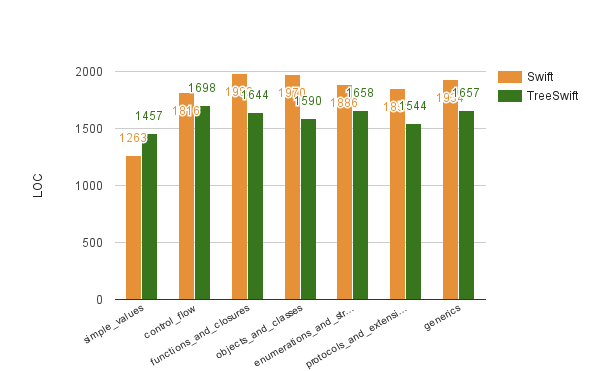
\includegraphics[scale=0.8]{./img/parse_loc_result.png}
        \caption{構文解析本体ファイルに対象を絞った実行部分LOC}
        \label{img:parse-loc-result}
    \end{center}
\end{figure}

\begin{figure}
    \begin{center}
        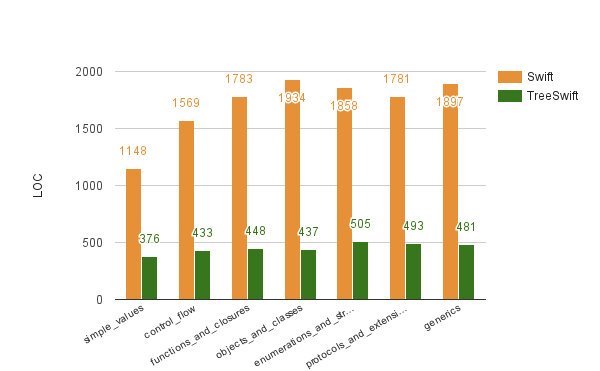
\includegraphics[scale=0.8]{./img/ast_loc_result.png}
        \caption{ASTファイルに対象を絞った実行部分LOC}
        \label{img:ast-loc-result}
    \end{center}
\end{figure}

\begin{table}[!hbtp]
    \begin{center}
        \caption{構文解析本体ファイルに対象を絞った実行部分LOCの差と比}
        \begin{tabular}{|p{0.45\linewidth}|p{0.225\linewidth}|p{0.225\linewidth}|}
            \hline
            対象プログラム & 差 & 比\\
            \hline
            \hline
            simple\_values.swift & -194 & 0.867\\
            \hline
            control\_flow.swift & 118 & 1.069\\
            \hline
            functions\_and\_closures.swift & 338 & 1.206\\
            \hline
            objects\_and\_classes.swift & 380 & 1.239\\
            \hline
            enumerations\_and\_structures.swift & 228 & 1.138\\
            \hline
            protocols\_and\_extensions.swift & 307 & 1.199\\
            \hline
            generics.swift & 277 & 1.167\\
            \hline
        \end{tabular}
        \label{table:parse-loc-arith}
    \end{center}
\end{table}

\subsection{考察}

まず、表~\ref{table:loc-result}の全体における実行部分LOCで両コンパイラに異様に大きな差を与えていた原因は表~\ref{table:loc-swift-per-file}の実行部分LOCを各ファイル種別ごとに分割して算出した結果から、構文解析本体ファイルではなく、その後の処理のための準備を行うためのプログラム群にあると考えられる。
実際、現行のSwiftコンパイラはその後に控えるSIL生成のためにASTを走査して正当性の確認を行ったり、Swiftプログラムの構文からSIL生成用の付帯情報が構文解析時に生成されるようにしており、それらのTreeSwiftに存在しない機能を提供するためのプログラムが実行部分LOCの大きな差を生んでいると見られる。
なお、表~\ref{table:loc-treeswift-per-file}においてTreeSwiftでの構文解析本体ファイルおよびASTファイル以外のファイルの実行部分LOCが同じ値となっているのは、TreeSwiftではそうした追加情報の生成やASTの正当性確認を行っておらず、その他のファイルがコンパイラ全体で使用されるファイルIOの仕組みなどを提供する基本ツールだけで構成されており、構文にかかわらず同じように使用されるからである。

しかし、図~\ref{img:parse-loc-result}にあるそうした部分を差っ引いた構文解析本体ファイルについてのみの結果を見ても、simple\_values.swift以外の例でTreeSwiftの方が低い実行部分LOCを記録している。
特にこの差を作り出していると考えられる原因の1つが、両コンパイラにおける分岐構文の使用傾向の差異である。
表~\ref{table:branching-method-swift}および表~\ref{table:branching-method-treeswift}は各対象プログラムを実行した際の構文解析本体ファイルにおいて実行された行(実行部分LOCの算出元となっている行)の内、現行のSwiftコンパイラではif文とswitch文とassert文、TreeSwiftではif文とswitch文とguard文がそれぞれ何度使用されているかをまとめたものである。

これらの表に見られる通り、現行のSwiftコンパイラにおいてはswitch文に対してif文が多く使用されているのに比べて、TreeSwiftではif文の使用量が減り、代わりにswitch文の使用量が増加している。
これは、Swiftの持つ強力なパターンマッチや列挙型によって、C++では異なる分岐文で別個に処理されていたものを同一のswitch文で使用できるようになったためだと考えられる。
Swiftのパターンマッチは条件判定と同時に列挙型やタプルなどの内部構造を分解して変数に束縛する役割を果たすため、switch文への移行は複数の条件文をまとめた上で変数の宣言や代入に関する行を削減することに繋がり、結果として実行部分LOCに減少につながっていたと考えられる。

また、simple\_values.swiftのみにおいてTreeSwiftの実行部分LOCが大きくなっていたのは、~\ref{implementation:abstract:parser}節で述べたように、TreeSwiftでは構文解析のステップを簡略化するために字句解析器が比較して複雑なアルゴリズムを採用しているためだと思われる。
これは、7つの対象プログラムについてSwiftの構文解析本体ファイルのみを対象とした実行部分LOCの標本分散は約53874であるのに対して、TreeSwiftでは約5930と低く、TreeSwiftの方が全てのプログラムで共通して実行されている部分が多くの部分を占めていることからも考察できる。

\begin{table}[!hbtp]
    \begin{center}
        \caption{Swiftにおける構文解析本体ファイルの実行部分中の分岐構文の行数}
        \begin{tabular}{|p{0.5\linewidth}|p{0.15\linewidth}|p{0.15\linewidth}|p{0.15\linewidth}|}
            \hline
            対象プログラム & if文 & switch文 & assert文\\
            \hline
            \hline
            simple\_values.swift & 266 & 22 & 33\\
            \hline
            control\_flow.swift & 392 & 28 & 43\\
            \hline
            functions\_and\_closures.swift & 432 & 28 & 46\\
            \hline
            objects\_and\_classes.swift & 449 & 28 & 37\\
            \hline
            enumerations\_and\_structures.swift & 407 & 26 & 38\\
            \hline
            protocols\_and\_extensions.swift & 407 & 27 & 35\\
            \hline
            generics.swift & 436 & 26 & 43\\
            \hline
        \end{tabular}
        \label{table:branching-method-swift}
    \end{center}
\end{table}

\begin{table}[!hbtp]
    \begin{center}
        \caption{TreeSwiftにおける構文解析本体ファイルの実行部分中の分岐構文の行数}
        \begin{tabular}{|p{0.5\linewidth}|p{0.15\linewidth}|p{0.15\linewidth}|p{0.15\linewidth}|}
            \hline
            対象プログラム & if文 & switch文 & guard文\\
            \hline
            \hline
            simple\_values.swift & 193 & 60 & 19\\
            \hline
            control\_flow.swift & 223 & 68 & 22\\
            \hline
            functions\_and\_closures.swift & 206 & 69 & 21\\
            \hline
            objects\_and\_classes.swift & 208 & 69 & 23\\
            \hline
            enumerations\_and\_structures.swift & 219 & 71 & 26\\
            \hline
            protocols\_and\_extensions.swift & 201 & 64 & 25\\
            \hline
            generics.swift & 214 & 70 & 26\\
            \hline
        \end{tabular}
        \label{table:branching-method-treswift}
    \end{center}
\end{table}

%%% Local Variables:
%%% mode: japanese-latex
%%% TeX-master: "../thesis"
%%% End:
